\documentclass[t]{beamer}
\usetheme{Warsaw}
\usecolortheme{seahorse}
\usepackage{array}
%\usepackage{graphicx}
\usepackage{amssymb,amsmath,mathrsfs,amsfonts}
%\usepackage[colorhighlight,display]{texpower}
%\usepackage{caption}
%\usepackage[all]{xy}
\usepackage{beamerthemesplit}
\mode<presentation>
%\usepackage{pause}
\usepackage{ulem}  % for strikethroughs
\usepackage{cancel} % for strikethroughs in math mode 
\usepackage{tikz}
\usetikzlibrary{shapes}
\usepackage{hyperref}
\hypersetup{pdfpagemode=FullScreen}
\usepackage{ifthen}
\usepackage{animate}
\usepackage{color}
\usepackage{type1cm}  % used for watermarking
\usepackage{eso-pic}  % used for watermarking


\theoremstyle{plain}
\newtheorem{prop}{Proposition}
\newtheorem{thm}[prop]{Theorem}
\newtheorem{lem}[prop]{Lemma}
\newtheorem{cor}[prop]{Corollary}
\theoremstyle{definition}
\newtheorem{dfn}{Definition}
\newtheorem{test}{Test}
\newtheorem{rem}[prop]{Remark}
\newtheorem{ex}{Example}[section]
%\newtheorem{note}{Note}[section]
\newtheorem{exercise}{Exercise}[section]
\newcommand{\nin}{\noindent}
\newcommand{\ds}{\displaystyle}
\renewcommand{\figurename}{Figure \arabic{figure}}



\renewcommand*\familydefault{\sfdefault} 




%%%%%%%%%%%%%%%%%%%%%%%%%%5
%%%%%%%%%%%%%%%%%%%%%%%%%%%%
%%%% some commands that have different meaning in the article/presentation modes

\newcommand{\vvfill}{\mode<presentation>{\vfill}  \mode<article>{\medskip}}   %vfill in presentation only
\newcommand{\sketchspace}{ 
\mode<article>{ \medskip\noindent{\textbf{Sketch:}} \vspace*{6cm} }
\mode<presentation>{ } 
}
\newcommand{\examplespace}{ 
\mode<article>{ \medskip\noindent{\textbf{Example:}} \vspace{6cm} }
\mode<presentation>{ } 
}
\newcommand{\artsmspace}{\mode<article>{\vspace*{2cm}} }  %small space in article mode
\newcommand{\artlargespace}{\mode<article>{\vspace*{6cm}} }  %large space in article mode

\newcommand{\dx}{\,dx}

\newcommand{\soln}{{\textbf{Solution: }}\,\,\,}
\newcommand{\disp}{\displaystyle}

\newcommand{\makedate}{\vvfill
\begin{picture}(10,10)  
\put(260,-20){\mbox{\tiny{\today}}}
\end{picture}
}

\newcommand{\pd}[2]{\dfrac{\partial#1}{\partial#2}}
\newcommand{\pD}[2]{\dfrac{\partial^2#1}{\partial#2^2}}
\newcommand{\pdd}[3]{\dfrac{\partial^2#1}{\partial#2 \partial#3}}


\normalem %stops the ulem package making all the emphs into underlines....
 
 
 
 \newcommand{\refandrev}[2]{
 \begin{small}
  \hspace{6cm}
  \begin{minipage}[r]{8cm}
  Stewart,    Chapter #1   \\
  Review:  \parbox[t]{6cm}{#2}
\end{minipage}
\end{small}
}



\newcounter{heading}
\setcounter{section}{1}
\setcounter{heading}{0}

\newcommand{\makeheading}[1]{\medskip\begin{large}\noindent\textbf{{#1}}\end{large}\smallskip}

%\newenvironment{head}[1]{\medskip\stepcounter{heading}\noindent\textbf{\hspace{0.2cm}{#1}.}}{}
\newcommand{\newhead}[1]{\medskip\stepcounter{heading}\noindent\textbf{\hspace{0.2cm}{#1}.}}


\newcommand{\pf}[1]{\noindent\textit{Proof.}\vspace*{#1 cm}}
\newcommand{\sol}[1]{\noindent\textit{Solution.}\vspace*{#1 cm}}
\newcommand{\further}[1]{\begin{small}\noindent\textit{Further reading: #1}\end{small}}
\newcommand{\exr}[1]{\begin{footnotesize}\noindent\textit{\textbf{Exercises:} Stewart #1}\end{footnotesize}}


% Sets of numbers
\newcommand{\C}{\mathbb{C}}
\newcommand{\RR}{\mathbb{R}}
\newcommand{\Z}{\mathbb{Z}}
\newcommand{\N}{\mathbb{N}}
\newcommand{\Q}{\mathbb{Q}}

% Partitions
\newcommand{\PP}{\mathcal{P}}

% Limits
\newcommand{\limm}[1]{\displaystyle \lim_{x\to #1}}

% Backslash
\newcommand{\bs}{\backslash}

% functions
\newcommand{\cosec}{\mathrm{cosec}}
\newcommand{\cosech}{\mathrm{cosech}}
\newcommand{\sech}{\mathrm{sech}}
\newcommand{\Li}{\mathrm{Li}}
\newcommand{\si}{\mathrm{Si}}
\newcommand{\erf}{\mathrm{erf}}

% Domain and Range
\newcommand{\Dom}{\mathrm{Dom}}
\newcommand{\Codom}{\mathrm{Codom}}
\newcommand{\Range}{\mathrm{Ran}}



\title{Week 4:  Related Rates,  Maxima,  Derivative Tests}
%\date{August 13 -- August 17, 2012}

\begin{document}

\frame{\titlepage}

\setcounter{tocdepth}{2}
\frame{\tableofcontents
}

\AtBeginSection[]
{
\begin{frame}<beamer> 
\tableofcontents[currentsection]  % show TOC and highlight current section
\end{frame}
}

\section{Related rates}

\begin{frame}
\frametitle{Related rates}

Related rates concern \textbf{real-world problems} related to \textbf{derivatives}.

\vspace{1em}

\textbf{Strategy} for solving related rates problems.
\begin{enumerate}
\item Draw a diagram
\item Assign variables
\item Express the problem in terms of derivatives
\end{enumerate}

\vspace{1em}

They are not easy, but the key is at least know that derivatives can be used to solve such problem.

\end{frame}


\begin{frame}

\footnotesize

\frametitle{Example}

A tornado is 20 km west of us, heading due east towards your house at a rate of 40 km/h.  You take your bicycle and ride due south at a speed of 12 km/h.  How fast is the distance between you and the tornado changing after 15 minutes?

\begin{figure}[t]
\begin{center}
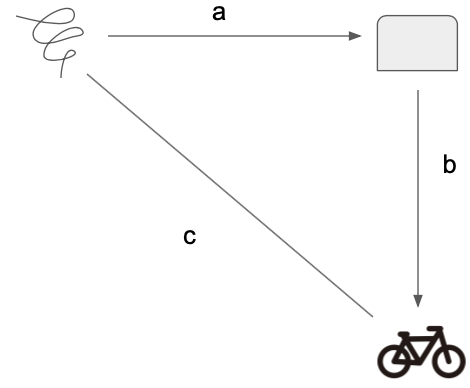
\includegraphics[scale=0.3]{fig/tornado}
\end{center}
\end{figure}

\end{frame}

\begin{frame}

\frametitle{Example}

\footnotesize

A tornado is 20 km west of us, heading due east towards your house at a rate of 40 km/h.  You take your bicycle and ride due south at a speed of 12 km/h.  How fast is the distance between you and the tornado changing after 15 minutes?

\vspace{-1em}

\begin{align*}
    a^2 + b^2 &= c^2 \\
    \dfrac{d}{dt}(a^2 + b^2) &= \dfrac{d}{dt} (c^2) \\
   2a* \dfrac{da}{dt} + 2b* \dfrac{db}{dt}  &= 2c* \dfrac{dc}{dt} \\
\end{align*}

\vspace{-1em}

$\dfrac{da}{dt} = -40; \dfrac{db}{dt} =12$,  when $t=0.25$ hrs, $a=10, b=3, c^2 = 10^2 + 3^2 = \sqrt{109}$ 

\begin{align*}
   2(10)*(-40) + 2(3)*2 &= 2 * \sqrt{109} * \dfrac{dc}{dt}  &&\\
   \dfrac{dc}{dt} &= -35 \text{km/h} 
\end{align*}	

\end{frame}

\begin{frame}
\footnotesize
\frametitle{Example}
Water flows into a tank at a rate of 3 cubic meters per minute. The tank is shaped like a cone with a height of 4 meters and a radius of 5 meters at the top.  Find the rate at which the water level is rising in the tank when the water height is 2 meters.   Find $\dfrac{dh}{dt}$.

\begin{figure}[t]
\begin{center}
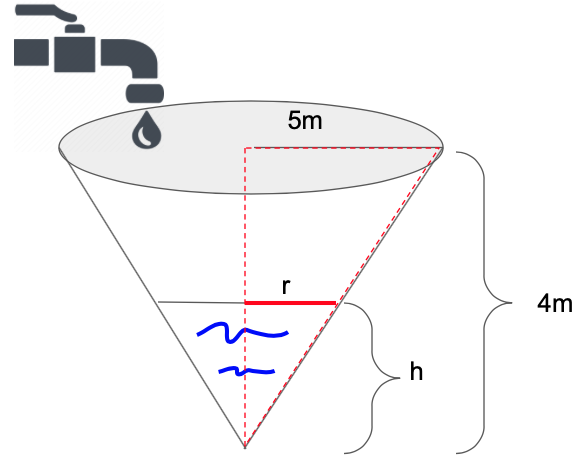
\includegraphics[scale=0.25]{fig/watertank}
\end{center}
\end{figure}

\end{frame}

\begin{frame}
\footnotesize
\frametitle{Example}
Water flows into a tank at a rate of 3 cubic meters per minute. The tank is shaped like a cone with a height of 4 meters and a radius of 5 meters at the top.  Find the rate at which the water level is rising in the tank when the water height is 2 meters.    Find $\dfrac{dh}{dt}$.

\begin{align*}
	V &= \dfrac{1}{3}\text{(area)}\text{(height)} = \dfrac{1}{3}\pi r^2 h\\
	&= \dfrac{1}{3}\pi \dfrac{25}{16} h^3 = \dfrac{25}{48}\pi h^3 && (\dfrac{r}{h} = \dfrac{5}{4}: \text{Properties of similar triangles}) \\
	\dfrac{dV}{dt} &= \dfrac{25}{48}\pi 3h^2 \dfrac{dh}{dt}\\
	3 &=  \dfrac{25}{48}\pi 3 (2)^2 \dfrac{dh}{dt}\\
	\dfrac{12}{25}\pi &=  \dfrac{dh}{dt} && (\text{meter per minute})\\
\end{align*}

\end{frame}

\begin{frame}
\frametitle{Self-Exercise}

\footnotesize

A ladder 10 ft long rests against a vertical wall.   If the bottom of the ladder slides away from the wall at a rate of 1 ft/s, how fast is the top of the ladder sliding down the wall when the bottom of the ladder is 6 ft from the wall?

\begin{figure}[t]
\begin{center}
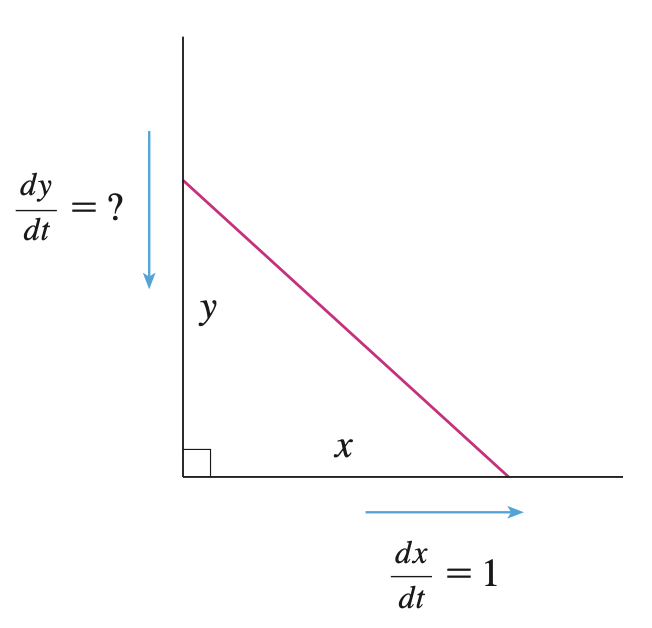
\includegraphics[scale=0.45]{fig/ladder}
\end{center}
\end{figure}

\end{frame}

\begin{frame}
\frametitle{Self-Exercise}

\footnotesize

A ladder 10 ft long rests against a vertical wall.   If the bottom of the ladder slides away from the wall at a rate of 1 ft/s, how fast is the top of the ladder sliding down the wall when the bottom of the ladder is 6 ft from the wall?

\begin{align*}
    x^2 + y^2 = 100\\
    2x\dfrac{dx}{dt} = 2y\dfrac{dy}{dt} &= 0\\
    \dfrac{dy}{dt} &= -\dfrac{x}{y} \dfrac{dx}{dt}\\
\end{align*}

When $x=6$,   $y=8$.  Also, we know $\dfrac{dx}{dt} = 1$, thus

$$\dfrac{dy}{dt} = -\dfrac{6}{8} * 1 = -\dfrac{3}{4} \text{ft/s} $$

\end{frame}

\section{Maxima and Minima}

\subsection{Definition}
\begin{frame}

\begin{dfn}
A function $f(x)$ has an \textbf{absolute maximum} at $x=c$ if $f(c) \geq f(x)$ for all $x$ in the \textbf{domain} of $f$.
\end{dfn}

\begin{dfn}
A function $f(x)$ has an \textbf{absolute minimum} at $x=c$ if $f(c) \leq f(x)$ for all $x$ in the \textbf{domain} of $f$.
\end{dfn}

\begin{dfn}
A function $f(x)$ has an \textbf{local (relative) maximum} at $x=c$ if $f(c) \geq f(x)$ for all $x$ \textbf{near} $c$.
\end{dfn}

\begin{dfn}
A function $f(x)$ has an \textbf{local (relative) minimum} at $x=c$ if $f(c) \leq f(x)$ for all $x$ \textbf{near} $c$.
\end{dfn}

\end{frame}


\begin{frame}

\frametitle{Example}

Where is the absolute minimum, maximum;  local minimum, maximum?

\begin{figure}[t]
\begin{center}
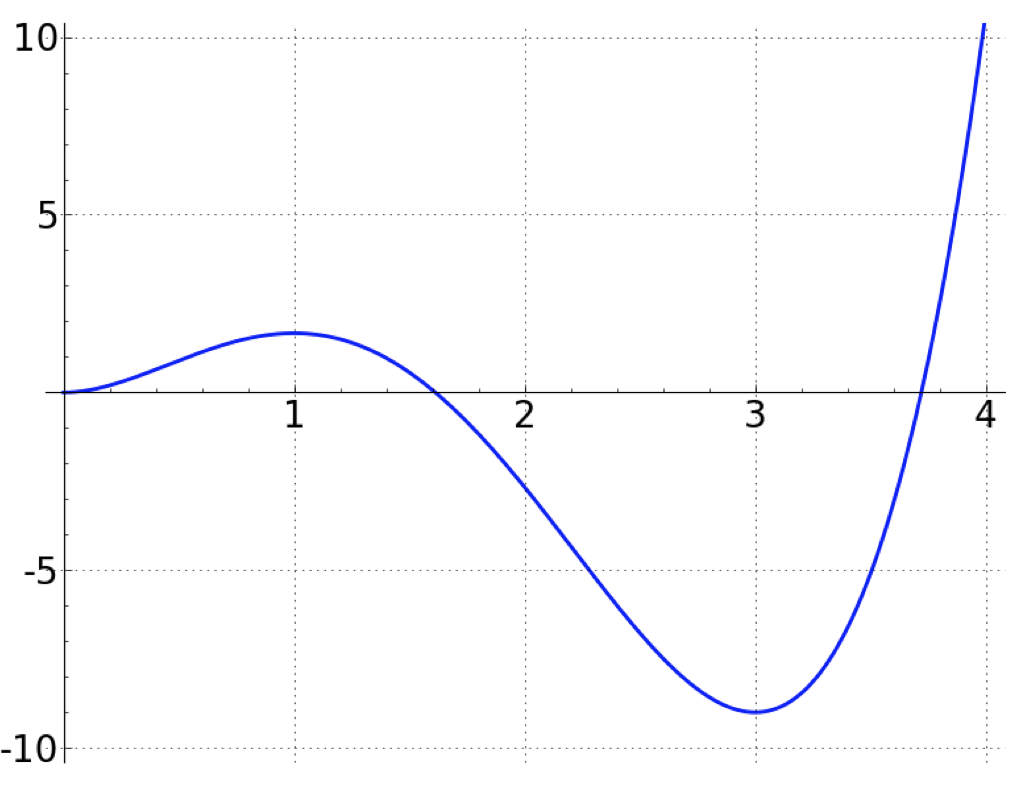
\includegraphics[scale=0.25]{fig/maxima}
\end{center}
\end{figure}

Abs. min: (3, -8)
Abs. max: (4, 10)\\
Local min: (3,-8)
Local max: (1, 2)\\
Note: (4,10) is NOT a local max because f(x) is not defined on an open interval around 4

\end{frame}

\begin{frame}

\frametitle{Exercise}

\footnotesize

Where is the absolute minimum, maximum;  local minimum, maximum?

\begin{figure}[t]
\begin{center}
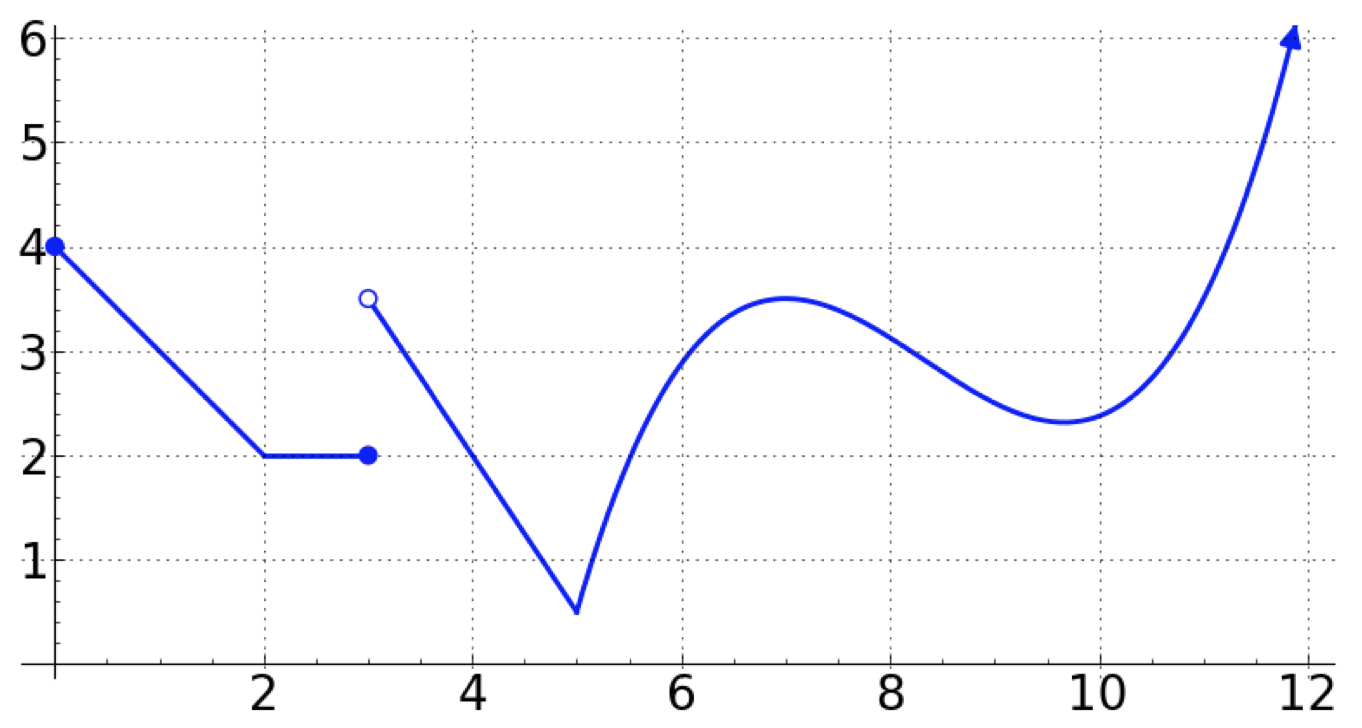
\includegraphics[scale=0.25]{fig/maxima2}
\end{center}
\end{figure}

\pause

Abs. min: (5, 0.5)\\
Abs. max: None because the graph keeps going up\\
Local min: (2, 2) to (3, 2);  (5, 0.5);  (9.8, 2,2)\\
Local max: (7, 3.5)\\
Note: (0,4) is NOT a local max because f(x) is not defined on an open interval \\
Note: (3,3.5) is NOT a local max because is not defined, and also, there is always a higher value if you keep close in on (3, 3.5)\\

\end{frame}

\subsection{Critical Number}

\begin{frame}

\frametitle{Critical Number}

\begin{dfn}
A number $c$ is critical number for a function $c$ if $f'(c)$ DNE or $f'(c) = 0$.
\end{dfn}

\begin{prop}
If $f$ has a local max or min at $x=c$, then $c$ must be a critical number for f. 

\vspace{1em}

If $c$ is a critical number, $f(c)$ may or may not be a local max or min (e.g.  $f(x) = x^3$ at $c=0$).
\end{prop}

\end{frame}

\begin{frame}

\frametitle{Example}

If $f$ has a local max or min at $x=c$, then $c$ must be a critical number for f. 

\begin{figure}[t]
\begin{center}
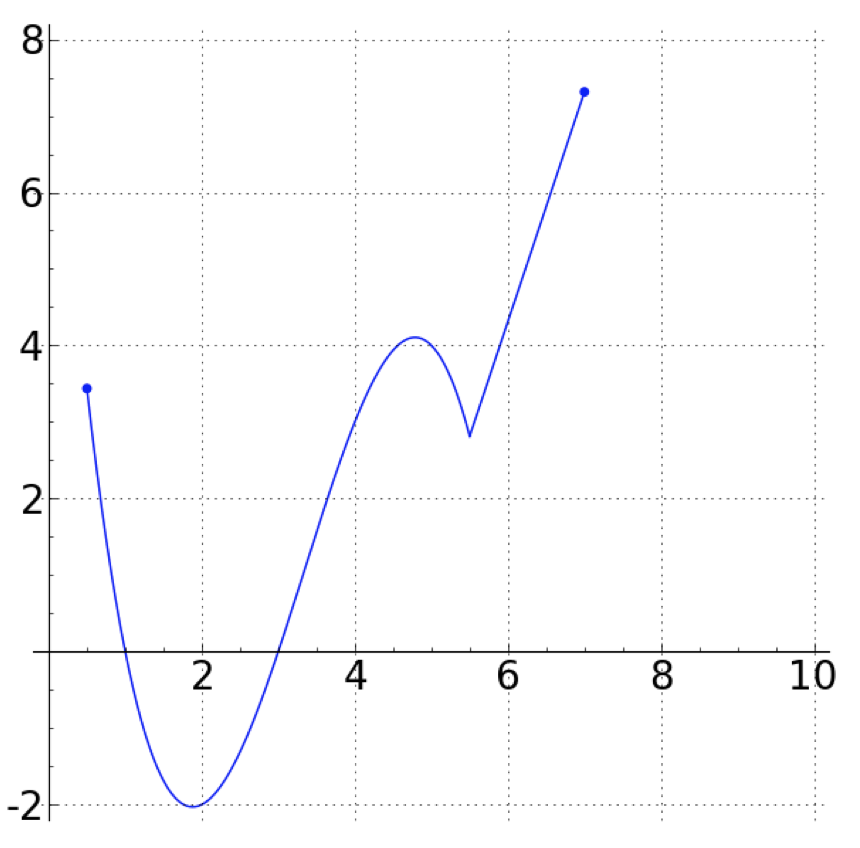
\includegraphics[scale=0.35]{fig/critical}
\end{center}
\end{figure}

\end{frame}

\begin{frame}

\frametitle{Example}

If $c$ is a critical number, $f(c)$ may or may not be a local max or min (e.g.  $f(x) = x^3$ at $c=0$).

\begin{figure}[t]
\begin{center}
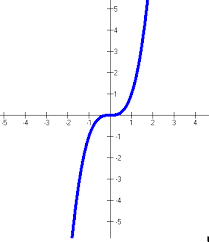
\includegraphics[scale=0.60]{fig/critical2}
\end{center}
\end{figure}

\end{frame}

\begin{frame}

\frametitle{Example}

Find critical numbers of $f(x) = x^{3/5} (4-x)$ \pause

\vspace{1em}

$f'(x) = \dfrac{12-8x}{5x^{2/5}}$

\vspace{1em}

Find $f'(x) = 0$ or $f'(x) = $DNE.

\vspace{1em}

$f'(x) = 0$ when $x = \dfrac{3}{2}$

\vspace{1em}

$f'(x) = $ DNE when $x = 0$

\end{frame}

\begin{frame}

\frametitle{Exercise}
\footnotesize

Find critical numbers of $g(t) = |3t-4|$ \pause

\vspace{1em}

 $g(t) = \begin{cases}
3t-4&\mbox{if }3t-4 \geq 0\\
-(3t-4)&\mbox{if }3t-4 < 0
\end{cases}$

 $g(t) = \begin{cases}
3t-4&\mbox{if }t \geq \dfrac{4}{3}\\
-(3t-4)&\mbox{if }t < \dfrac{4}{3}
\end{cases}$

 $g'(t) = \begin{cases}
3&\mbox{if }t \geq \dfrac{4}{3}\\
-3&\mbox{if }t < \dfrac{4}{3}
\end{cases}$

Since the derivative is a sharp corner at $\dfrac{4}{3}$, thus $f'(\dfrac{4}{3}) = $DNE, thus $\dfrac{4}{3}$ is the critical number.

\end{frame}

\begin{frame}

\frametitle{Absolute Maximum/Minimum}

\begin{prop}[The Closed Interval Method]
To find the absolute maximum and minimum values (also called extreme values) of a continuous function $f$ on a closed interval [a,b]:
\begin{enumerate}
	\item Find the values of $f$ at the critical numbers of $f$ in $[a, b]$.
	\item Find the values of $f$ at the endpoints of the interval.
	\item The largest of the values from Steps 1 and 2 is the absolute maximum value; the smallest of these values is the absolute minimum value.
\end{enumerate}
\end{prop}

\end{frame}

\begin{frame}

\frametitle{Example}

Find the absolute minimum and maximum of $f(x) = x^3 - 3x^2 + 1$ in $[-\dfrac{1}{2}, 4]$\pause

\begin{itemize}
	\item $f'(x) = 3x(x-2)$
	\item The critical numbers are 0 and 2
	\item The values at critical numbers \textit{inside the interval} are $f(0) = 1$ and $f(2) = -3$
	\item The values at endpoints are $f(-\dfrac{1}{2})=\dfrac{1}{8}$ and $f(4) = 17$
	\item Comparing these four numbers, $f(4)=17$ is the absolute max, and $f(2)=-3$ is the absolute min.
\end{itemize}

\end{frame}

\begin{frame}

\frametitle{Exercise}

Find the absolute minimum and maximum of $f(x) = \dfrac{x-1}{x^2+x+2}$ in $[0, 4]$\pause

\begin{itemize}
	\item $f'(x) = \dfrac{-x^2+2x+3}{(x^2+x+2)^2}$
	\item The critical numbers are 3 and -1
	\item The values at critical numbers \textit{inside the interval} is $f(3) = \dfrac{1}{7}$
	\item The values at endpoints are $f(0)=-\dfrac{1}{2}$ and $f(4) = \dfrac{3}{22}$
	\item Comparing these three numbers, $f(3) = \dfrac{1}{7}$ is the absolute max, and $f(0)=-\dfrac{1}{2}$ is the absolute min.
\end{itemize}

\end{frame}

\subsection{Mean Value Theorem}

\begin{frame}
\frametitle{The Mean Value Theorem}

\begin{theorem}[The Mean Value Theorem]
Let $f$ be a function that satisfies the following hypotheses:
\begin{enumerate}
\item $f$ is continuous on the closed interval $[a,b]$.
\item $f$ is differentiable on the open interval $(a,b)$.
\end{enumerate}
Then there is a number $c$ in $(a,b)$ such that
\[f'(c) = \frac{f(b) - f(a)}{b-a}, \quad \text{equivalently} \quad f(b) - f(a) = f'(c)(b-a).\]
\end{theorem}

\end{frame}

\begin{frame}

\frametitle{Example}

\begin{figure}[t]
\begin{center}
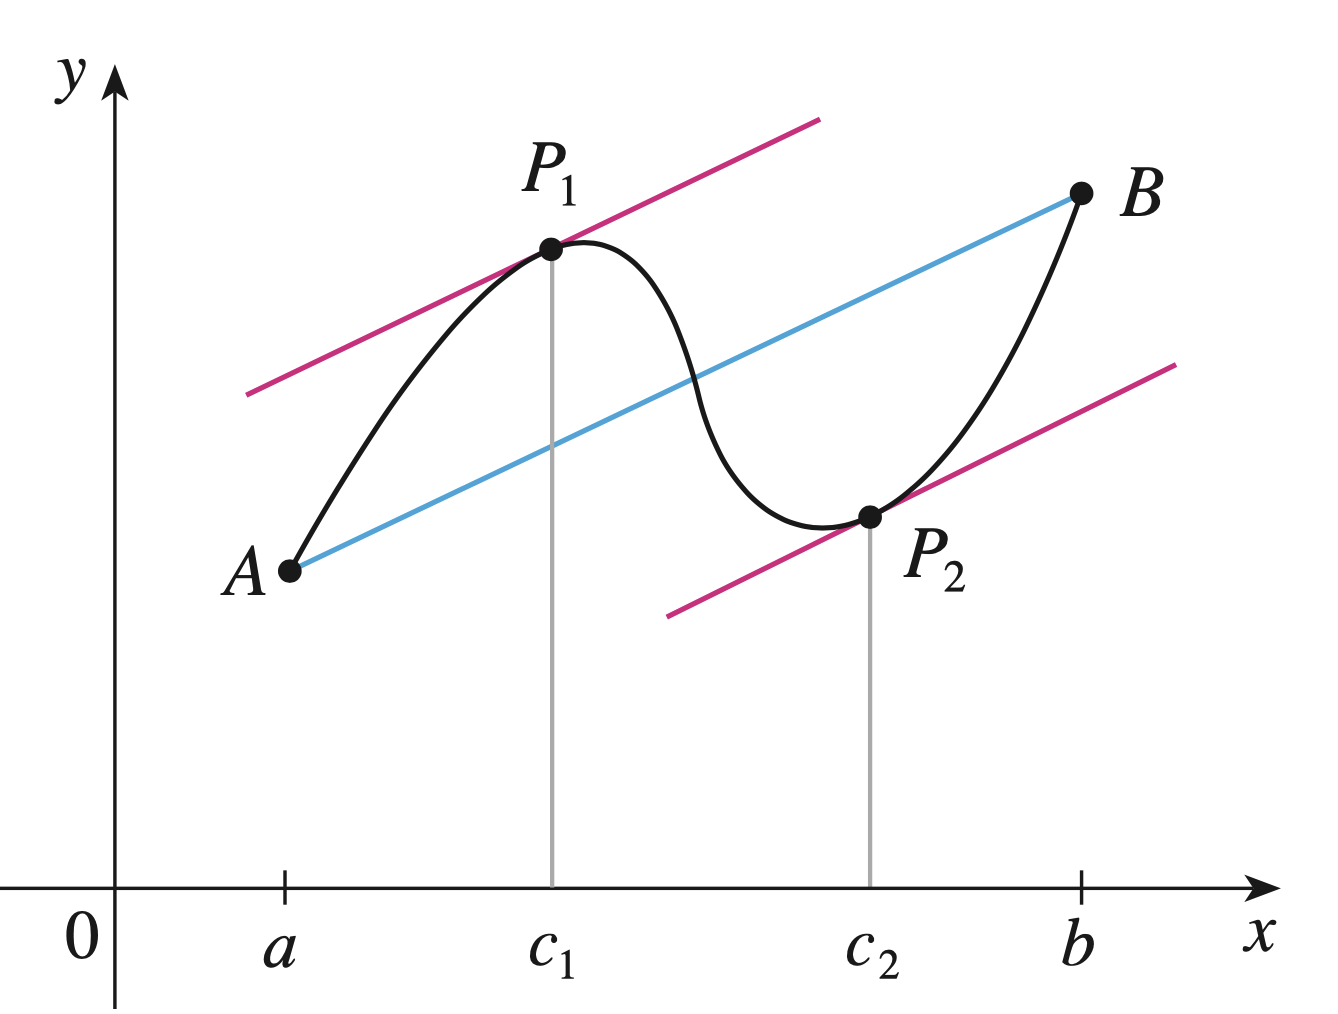
\includegraphics[scale=0.3]{fig/mvt}
\end{center}
\end{figure}

\end{frame}

\begin{frame}

\frametitle{Example}

\footnotesize

Verify the mean value theorem for $f(x) = 2x^3 - 8x + 1$ on the interval $[1, 3]$. \pause

\begin{itemize}
	\item $f$ is cont on $[1, 3]$
	\item $f$ is differentiable on $(1, 3)$
\end{itemize}

Find $c$ in [1, 3] such that $f'(c) = \dfrac{f(3) - f(1)}{3-1}.$

\begin{align*}
	f'(c) &= \dfrac{f(3) - f(1)}{3-1}\\
	6c^2 - 8  &= \dfrac{31-(-5)}{2}\\
	6c^2 - 8 &= 18\\
	6c^2 &= 24\\
	c^2 &= 4 = \pm 2
\end{align*}

$c=2$ is the answer because it falls inside the interval $[1, 3]$.

\end{frame}

\begin{frame}

\frametitle{Example}

\footnotesize

If $f$ is a differentiable function and $f(1) = 7$ and $-3 \leq f'(x) \leq -2$ on the interval $[1, 6]$, then what is the biggest and smallest values that are possible for $f(6)$?
\pause
\vspace{1em}

The MVT tells us that $\dfrac{f(6) - f(1)}{6-1} = f'(c)$ for some $c$ in $[1, 6]$.

\vspace{1em}

Thus we know that $-3 \leq \dfrac{f(6) - f(1)}{6-1} \leq -2$.

\vspace{1em}

We can replace $f(1) = 7$ and get $-3 \leq \dfrac{f(6) - 7}{6-1} \leq -2$.

\vspace{1em}

Solving this, we find that $-8 \leq f(6) \leq -3$.  

\end{frame}

\subsection{Rolle's Theorem}

\begin{frame}
\frametitle{Rolle's Theorem}

\begin{theorem}[Rolle's Theorem]
Let $f$ be a function that satisfies the following hypotheses:
\begin{enumerate}
\item $f$ is continuous on the closed interval $[a,b]$.
\item $f$ is differentiable on the open interval $(a,b)$.
\item $f(a) = f(b)$.
\end{enumerate}
Then there is a number $c$ in $[a,b]$ such that $f'(c)=0$
\end{theorem}

\end{frame}


\begin{frame}

\frametitle{Example}

\begin{figure}[t]
\begin{center}
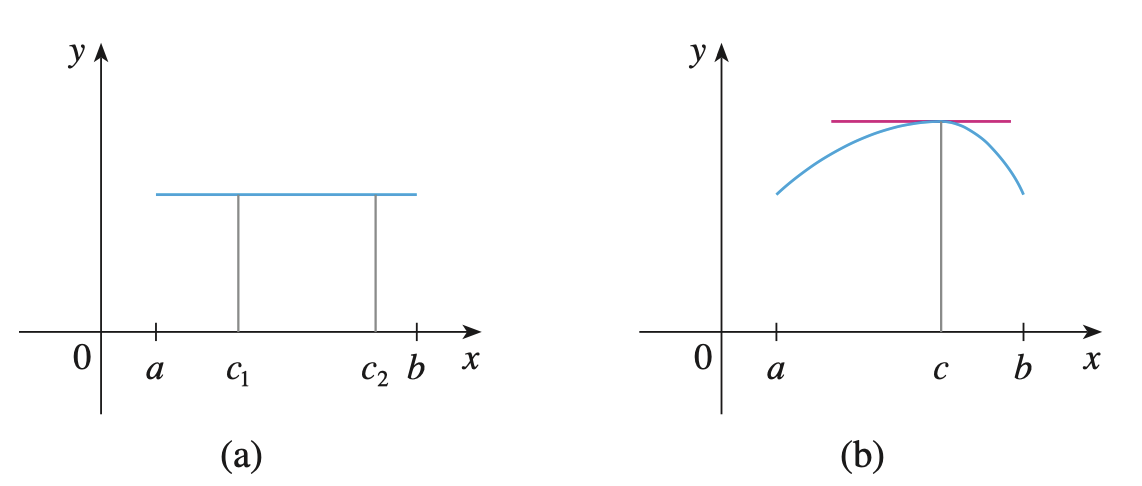
\includegraphics[scale=0.35]{fig/rolle1}
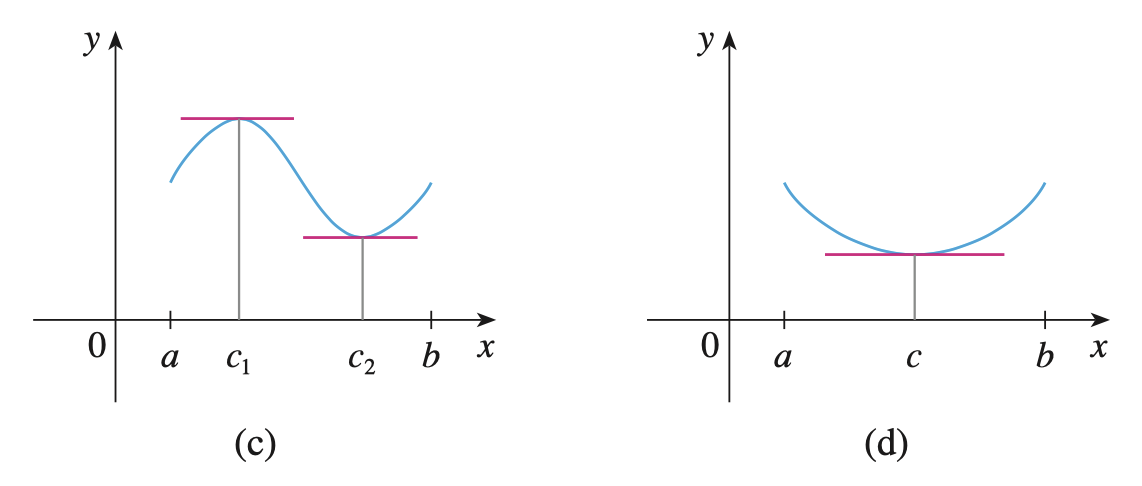
\includegraphics[scale=0.35]{fig/rolle2}
\end{center}
\end{figure}

\end{frame}


\section{Derivatives and Shapes of Graphs}

\subsection{Increasing/Decreasing Test}
\begin{frame}
\frametitle{Increasing/Decreasing Test}
\footnotesize
\begin{test}[Increasing/Decreasing Test]
	\begin{itemize}
		\item If $f'(x) > 0$ on an interval, then $f$ is increasing on that interval.
		\item If $f'(x) < 0$ on an interval, then $f$ is decreasing on that interval.
	\end{itemize}
\end{test}

\centering
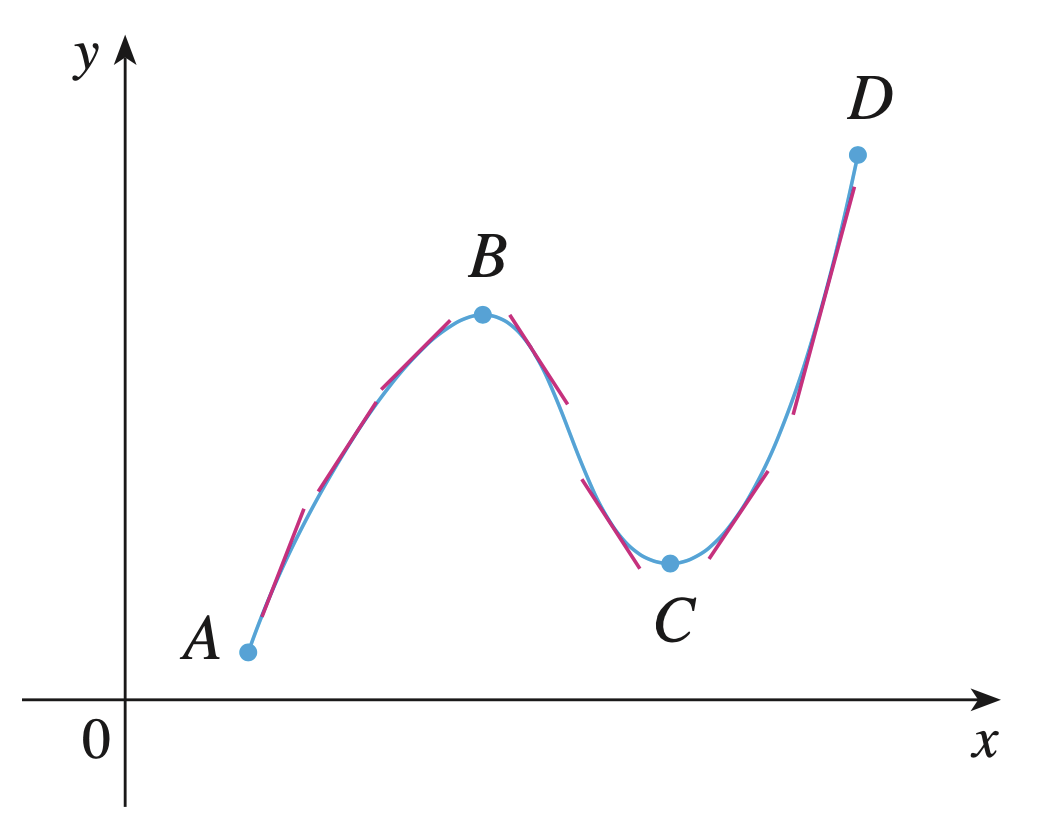
\includegraphics[scale=0.3]{fig/increasingtest}

\end{frame}

\subsection{First Derivative Test}
\begin{frame}
\frametitle{First Derivative Test}
\footnotesize
\begin{test}[First Derivative Test]
Suppose that $c$ is a critical number of a continuous function $f$.
	\begin{itemize}
		\item If $f'$changes from positive to negative at c, then $f$ has a local max at $c$.
		\item If $f'$changes from negative to positive at c, then $f$ has a local min at $c$.
		\item If $f'$ is positive or negative to the left and right of $c$, $f$ has no local max or min at $c$.
	\end{itemize}
\end{test}

\vspace{1em}
\centering
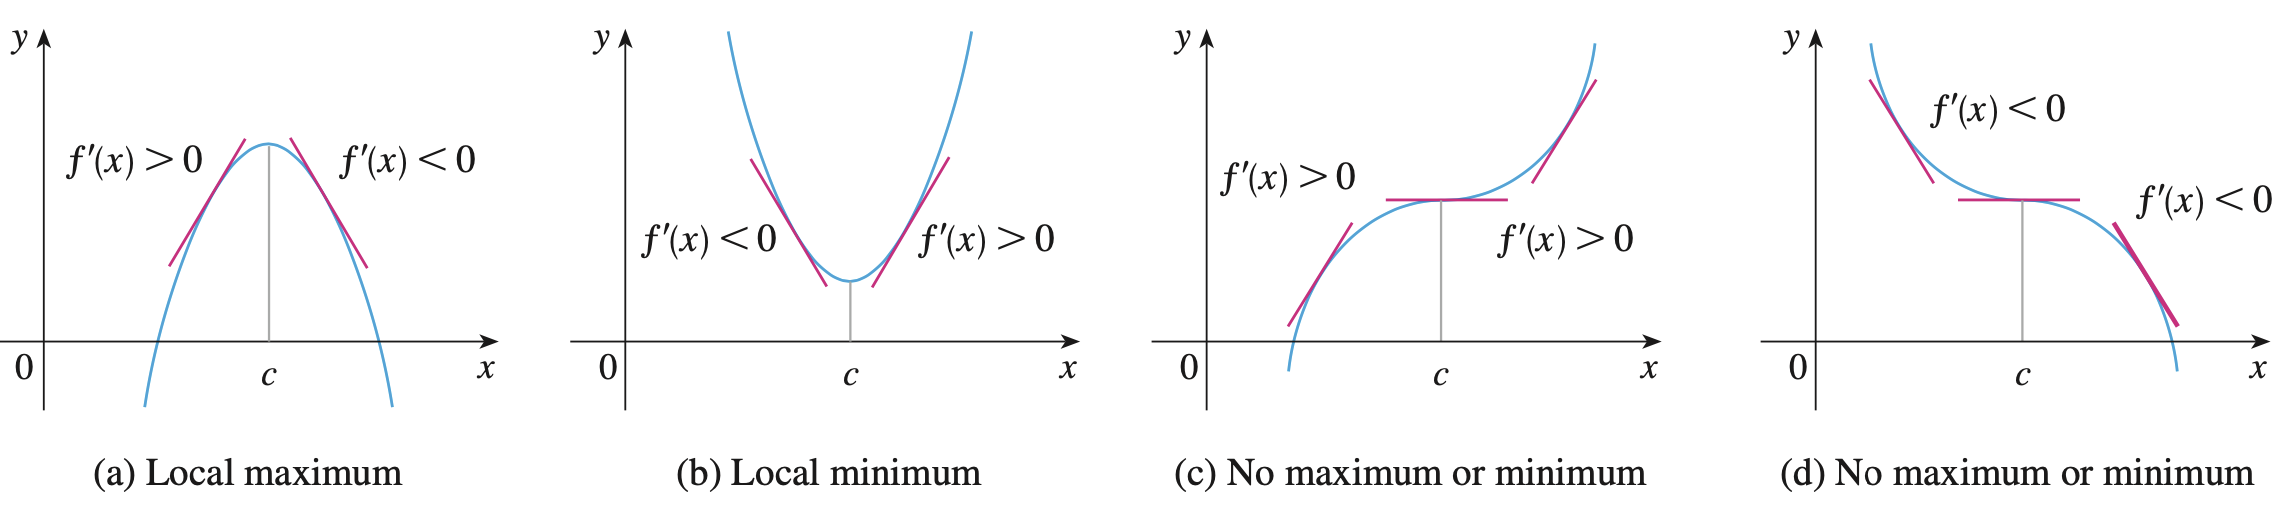
\includegraphics[scale=0.27]{fig/firsttest}

\end{frame}

\subsection{Concavity Test}
\begin{frame}
\frametitle{Concavity Test}
\footnotesize
\begin{test}[Concavity Test]
	\begin{itemize}
		\item If $f''(x) > 0$ for all $x$ in an interval, then the graph of $f$ is concave upward on the interval
		\item If $f''(x) < 0$ for all $x$ in an interval, then the graph of $f$ is concave download on the interval
	\end{itemize}
\end{test}

\vspace{1em}
\centering
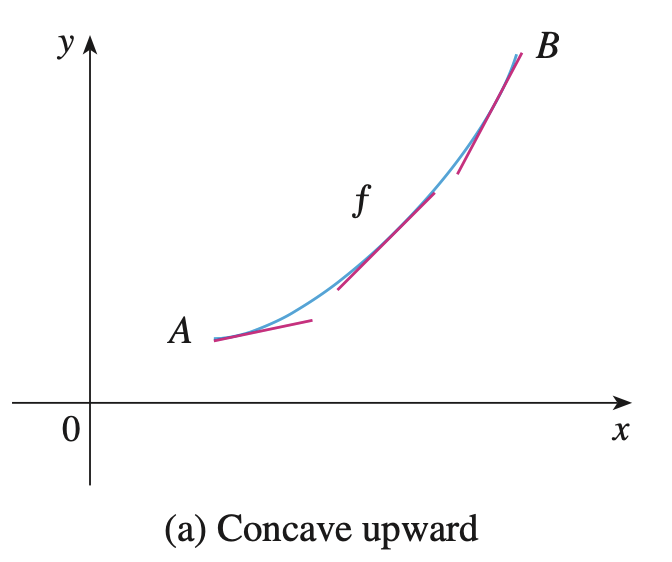
\includegraphics[scale=0.32]{fig/concave1}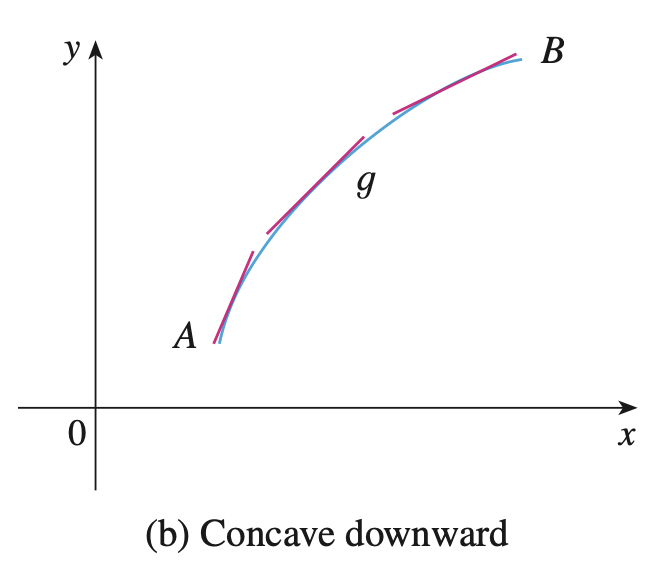
\includegraphics[scale=0.32]{fig/concave2}

\end{frame}

\subsection{Second Derivative Test}
\begin{frame}
\frametitle{Second Derivative Test}
\footnotesize
\begin{test}[Second Derivative Test]
Suppose $f''$ is continuous near $c$
	\begin{itemize}
		\item If $f'(c) = 0$ and $f''(c) > 0$, then $f$ has a local min at $c$.
		\item If $f'(c) = 0$ and $f''(c) < 0$, then $f$ has a local max at $c$.
	\end{itemize}
\end{test}

\vspace{1em}
\centering
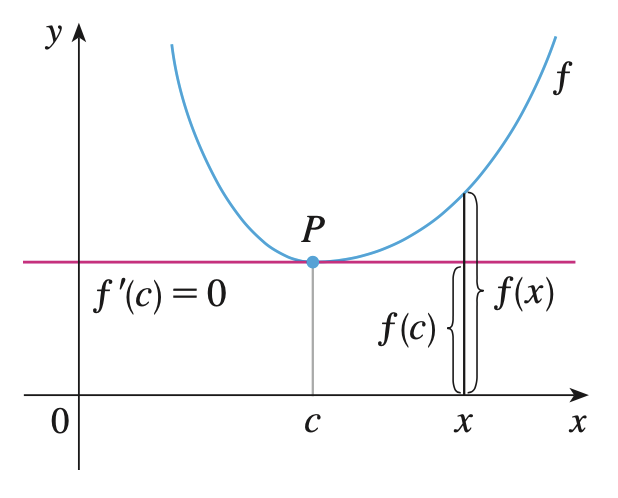
\includegraphics[scale=0.40]{fig/secondtest}

\end{frame}

\begin{frame}
\frametitle{Example}

Given $f(x) = x^3 - 3x^2 - 9x + 4$,  (1) Find intervals on which $f$ is increasing or decreasing.  (2) Find the local max and min.  (3) Find the intervals of concavity. \pause

\vspace{1em}

$f'(x) = 3(x + 1)(x-3)$ and $f''(x) = 6(x-1)$

\begin{enumerate}
		\item After trying some values on $f'(x)$ in the interval $(-\infty, -1), (-1, 3), (3, \infty)$, we will find that $f$ is increasing on $(-\infty, -1), (3, \infty)$ and decreasing on $(-1, 3)$
		\item $f$ changes from increasing to decreasing at $x=-1$, and from decreasing to increasing at $x=3$.  Thus $f(-1) = 9$ is a local max, and $f(3) = -23$ is a local min.
		\item Since $f''(x) > 0$ when $x >1$ and $f''(x) < 0$ when $x < 1$, thus $f$ is concave upward on $(1, \infty)$ and downward on $(-\infty, 1)$.
\end{enumerate}

\end{frame}

\begin{frame}

\frametitle{Exercise}

Given $f(x) = 2x^3 - 9x^2 +12x -3$,  (1) Find intervals on which $f$ is increasing or decreasing.  (2) Find the local max and min.  (3) Find the intervals of concavity.\pause

$f'(x) = 6(x - 1)(x - 2)$ and $f''(x) = 12(x-\dfrac{3}{2})$

\begin{enumerate}
		\item $f$ is increasing on $(-\infty, 1), (2, \infty)$ and decreasing on $(1, 2)$
		\item $f$ changes from increasing to decreasing at $x=1$, and from decreasing to increasing at $x=2$.  Thus $f(1) = 2$ is a local max, and $f(2) = 1$ is a local min.
		\item Since $f''(x) > 0$ when $x >\dfrac{3}{2}$ and $f''(x) < 0$ when $x < \dfrac{3}{2}$, thus $f$ is concave upward on $(\dfrac{3}{2}, \infty)$ and downward on $(-\infty, \dfrac{3}{2})$.
\end{enumerate}

\end{frame}

\begin{frame}
\frametitle{Example}

Given $f(x) = 1 + 3x^2 - 2x^3$,  find local max and min using (1) First Derivative Test, and (2) Second Derivative Test. \pause

\vspace{1em}

$f'(x) = 6x (1-x)$ and $f''(x) = 6 - 12x$

\begin{enumerate}
	\item $f'(x) > 0$ when $0 < x < 1$ and $f'(x) < 0$ when $x<0$ or $x>1$.  Since $f'$ changes from negative to positive at $x=0$, $f(0) = 1$ is a local min.   Since $f'$ changes from positive to negative at $x=1$, $f(1)=2$ is a local max.
	\item $f'(x) = 0$ when $x=0,1$.    Since $f''(0) = 6 > 0$, $f(0) = 1$ is a local min.   Since $f''(1) = -6 < 0$, $f(1) = 2$ is a local max. 
\end{enumerate}

\end{frame}

\begin{frame}

\frametitle{Exercise}

Given $f(x) = \dfrac{x^2}{x-1}$,  find local max and min using (1) First Derivative Test, and (2) Second Derivative Test. \pause

\vspace{1em}

$f'(x) = \dfrac{x(x-2)}{(x-1)^2}$ and $f''(x) = \dfrac{2}{(x-1)^3}$

\begin{enumerate}
	\item $f'(x) > 0$ when $x < 0$ or $x > 2$ and $f'(x) < 0$ when $0 < x < 1$ or $1 < x < 2$.  Since $f'$ changes from positive to negative at $x=0$, $f(0) = 0$ is a local max.   Since $f'$ changes from negative to positive at $x=2$, $f(2)=4$ is a local min.
	\item $f'(x) = 0$ when $x=0,2$.    Since $f''(0) = -2  < 0$, $f(0) = 0$ is a local max.   Since $f''(2) = 2 > 0$, $f(2) = 4$ is a local min. 
\end{enumerate}


\end{frame}





\end{document}
